\chapter{Fundamentação teórica}
\label{cap:fundamentacao-teorica}

Neste capítulo apresentaremos os conceitos centrais que serviram como base e guia para a elaboração deste trabalho. Ao início é falado sobre o conhecimento básico sobre compiladores, depois sobre o \textit{framework} utilizado para construção da ferramenta e por fim, sobre a tecnologia usada para fazer a integração com o \textit{Moodle}.

\section{Compiladores}
Programas que são executados em computadores são escritos no que é chamada de linguagem de máquina que usa comandos simples que são interpretados pela máquina. Escrever em linguagem de máquina é uma tarefa passível de erro e cansativa, e por essa razão foram criados os compiladores. Os compiladores traduzem linguagens de alto nível em linguagem de máquina e indicam erros cometidos pelos programadores no código-fonte \cite{mogensen2024introduction}.

\subsection{Fases do compilador}
As fases de um compilador podem ser divididas de várias formas. Os trabalhos de \textcite{cooper2022engineering,mogensen2024introduction, thain2020introduction} dão suas definições das fases de um compilador, mas para esse trabalho será seguida a definição de \textcite{thain2020introduction}.

\begin{figure}[ht]
    \captionsetup{width=16cm}
    \Caption{\label{fig:compfases}Fases de um compilador UNIX}
    \tcbox[left=0cm, right=0cm, top=0cm, bottom=0cm,center]{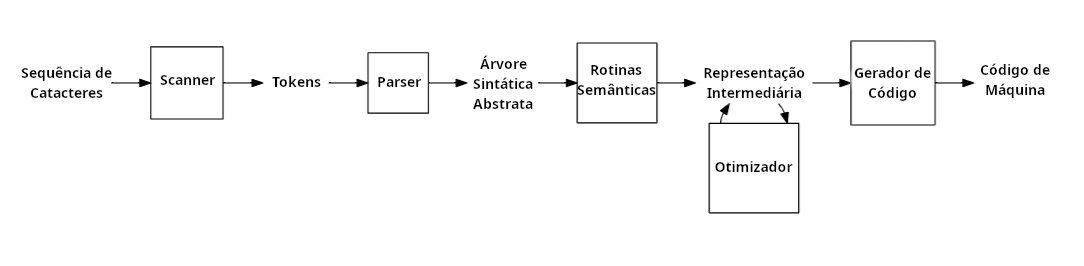
\includegraphics[width=15.6cm]{figuras/compfases.png}}{
        \Fonte{adaptada de \textcite{thain2020introduction}.}}
\end{figure}

\subsubsection{Análise Léxica}
Na fase de análise léxica, o \textit{scanner}, também chamado de \textit{tokenizer}, consome texto simples de um programa e agrupa os caracteres individuais em sequências chamadas de \textit{tokens}. Esse processo funciona de forma parecida com agrupar letras para formar palavras da linguagem natural, esse agrupamento é feito usando expressões regulares implementadas através de autômatos.

\subsubsection{Análise Sintática}
Análise de sintática será o foco do trabalho sendo discutida de forma mais aprofundada nas próximas seções. A fase de análise sintática da compilação rearranja os \textit{tokens} gerados pela fase de análise léxica, gerando assim uma estrutura chamada árvore sintática. Árvores sintáticas são estruturas de árvore como diz o nome, as folhas dessa árvore são os \textit{tokens} e a leitura em ordem da árvore dá a sequência de \textit{tokens} do texto de entrada dado ao analisador sintático. Ao construir a árvore sintática, o analisador sintático também checa se há erros de sintaxe no texto de entrada.

\subsubsection{Análise semântica}
Na fase de análise semântica, as rotinas semânticas percorrem a árvore sintática e buscam significado na entrada a partir das regras da gramática e da relação entre os elementos da entrada. Depois das rotinas semânticas, a árvore de análise sintática é convertida em uma representação intermediária que é uma versão simplificada de \textit{assembly} que permite uma análise detalhada.

\subsubsection{Otimização}
Na fase de otimização, otimizadores são aplicados na representação intermediária para tornar o programa mais rápido, menor e eficiente. Normalmente os otimizadores recebem uma entrada em formato de representação intermediária e retornam um resultado no mesmo formato para que todos os otimizadores possam ser aplicados de forma independente e em qualquer ordem.

\subsubsection{Geração de código}
Na fase de geração de código, o gerador de código consome a representação intermediária otimizada e a transforma em um programa em \textit{assembly} concreto. Para otimizar o uso dos registradores físicos limitados e gerar instruções de montagem de maneira eficiente, o gerador de código precisa executar as tarefas de alocação de registradores, seleção de instruções e sequenciamento de instruções.

\section{Analisadores Sintáticos Descendentes}
\textcite{cooper2022engineering,mogensen2024introduction, thain2020introduction} falam sobre analisadores sintáticos descendentes, mas para esse trabalhos será seguida a definiçã de \textcite{thain2020introduction}. Analisadores sintáticos descendentes, também chamados \textit{parsers top-down}, são métodos de análise sintática que iniciam a análise a partir do símbolo inicial da gramática. Eles fazem comparações entre os \textit{tokens} do texto de entrada e os símbolos da gramática para encontrar a produção que deve ser escrita no lugar dos símbolos da gramática. Essas comparações são feitas até sobrar apenas símbolos terminais, esses símbolos terminais devem coincidir com a sequência de \textit{tokens} da entrada caso contrário será considerado um erro.

\subsection{Descendentes Recursivos}
O conjunto de gramáticas que pode ser analisados usando algoritmos usando apenas um não terminal e o próximo símbolo da entrada é chamado conjunto de gramáticas LL(1). Uma das formas de fazer a análise dessas gramáticas é usando o analisador sintático descendente recursivo que usa funções recursivas para cada não terminal para processar a entrada. É um algoritmo que funciona como uma forma recursiva dos analisadores sintáticos LL(1) que já são tratados nesse trabalho, além disso, esse algoritmo não segue estruturas fixas e determinísticas, por isso não será abordado na ferramenta.

\subsection{Analisadores Sintáticos LL(1)}
Analisadores sintáticos LL(1) são um tipo de analisador sintático descendente, esses analisadores sintáticos levam em consideração um único \textit{lookahead} que nesse algoritmo é o símbolo inicial do lado direito das produções. O \textit{lookahead} é usado para decidir qual produção deve ser escrita, por essa razão apenas gramaticas não ambíguas podem ser analisadas pelos analisadores sintáticos LL(1).

O conjunto dos símbolos iniciais das produções de uma gramática é chamado conjunto \textit{first}. No algoritmo LL(1) o conjunto \textit{lookahead} corresponde ao conjunto \textit{first}, a construção desse conjunto pode ser feita seguindo o Algoritmo \ref{alg:first}. As definições dos algoritmos foram tiradas do trabalho de \textcite{thain2020introduction}.

\begin{algorithm}[ht]
    \caption{First}\label{alg:first}
    \Input{Gramática $G$, Símbolo $X$}
    \Output{Conjunto $\mathit{first}$}
    \Inicio{
        $\mathit{first} \gets \varnothing$ \\

        \Ifx{$X$ é terminal}{
            $\mathit{first} \gets \{ X \}$
        }
        \Elsex{
            \Repeat{não haja mais mudanças}{
                \ForEach{regra $X \rightarrow Y_1 Y_2 \dots Y_k$ em $G$}{
                    \Ifx{
                        $a \in \textsc{First}(Y_1) \lor (a \in \textsc{First}(Y_n) \land Y_1 \dots Y_{n-1} \Rightarrow^* \epsilon)$
                    }{
                        $\mathit{first} \gets \mathit{first} \cup \{ a \}$
                    }
                    \Ifx{$Y_1 \dots Y_k \Rightarrow^* \epsilon$}{
                        $\mathit{first} \gets \mathit{first} \cup \{ \epsilon \}$
                    }
                }
            }
        }
        \Return{$\mathit{first}$}
    }
\end{algorithm}

O conjunto \textit{follow} é o conjunto de símbolos terminais da gramática que podem ocorrer depois de qualquer uma das derivações de um não terminal \selectlanguage{brazil}$A$\selectlanguage{brazil}, o conjunto também inclui o símbolo \$ usado para se referir ao fim da \textit{string}. Esse conjunto é usado no analisador LL para lidar com produções que derivam uma \textit{string} vazia. A construção do conjunto \textit{follow} pode ser feita seguindo o Algoritmo \ref{alg:follow}.

\begin{algorithm}[ht]
    \caption{Follow}\label{alg:follow}
    \Input{Gramática $G$}
    \Output{Dicionário $\mathit{follow}$}
    \Inicio{
        $\mathit{follow} \gets \text{Dicionário}\langle\text{Símbolo}, \text{Conjunto}\rangle$ \\
        $\mathit{follow}[S] \gets \{ \$ \}$, {Onde $S$ é o símbolo inicial}

        \Repeat{até não haver mudanças}{
            \ForEach{produção $A \rightarrow \alpha$ em $G$}{
                \Ifx{$A \rightarrow \alpha B \beta$}{
                    $\mathit{follow}[B] \gets \mathit{follow}[B] \cup \left( \textsc{First}(\beta) - \{ \epsilon \} \right)$
                }
                \Ifx{$A \rightarrow \alpha B \lor \epsilon \in \textsc{First}(\beta)$}{
                    $\mathit{follow}[B] \gets \mathit{follow}[B] \cup \mathit{follow}[A]$
                }
            }
        }
        \Return{$\mathit{follow}$}
    }
\end{algorithm}

Uma tabela de análise sintática LL(1) pode ser usada para determinar as regras a serem usadas na análise de uma trada para todas as combinações de não terminais e \textit{tokens} da entrada. A construção dessa tabela pode ser feita usando os conjuntos de \textit{first} e \textit{follow} usando o Algoritmo \ref{alg:lltable}. Tendo a tabela de análise sintática LL(1) em mãos, é possível fazer a análise de uma sequência de \textit{tokens} usando uma \textit{stack}. O Algoritmo \ref{alg:llparse} mostra a análise sintática usando a tabela.

\begin{algorithm}[htp]
    \caption{Construção da Tabela LL(1)}\label{alg:lltable}
    \Input{Gramática $G$}
    \Output{Tabela $M$}
    \Inicio{
        $\mathit{follow} \gets \textsc{Follow}(G)$ \\
        \ForEach{regra $A \rightarrow \alpha$ em $G$}{
            \ForEach{terminal $a \in \textsc{First}(\alpha) - \{ \epsilon \}$}{
                $M[A, a] \gets (A \rightarrow \alpha)$
            }
            \Ifx{$\epsilon \in \textsc{First}(\alpha)$}{
                \ForEach{terminal $b \in \mathit{follow}[A]$}{
                    $M[A, b] \gets (A \rightarrow \alpha)$
                }
            }
        }
    }
\end{algorithm}
\begin{algorithm}[htp]
    \caption{Análise LL(1)}\label{alg:llparse}
    \Input{Gramática $G$, Tabela $M$}
    \Inicio{
        $\mathit{pilha} \gets [\$, S]$, {Onde $S$ é o símbolo inicial} \\
        $\mathit{token} \gets \text{pr\'oximo token}$ \\
        \While{$\mathit{pilha} \neq \varnothing$}{
            $X \gets \text{topo}(\mathit{pilha})$ \\
            \If{$X$ é terminal}{
                \If{$X = \mathit{token}$}{
                    $\text{desempilhe}(\mathit{pilha})$ \\
                    $\mathit{token} \gets \text{pr\'oximo token}$
                }
                \Elsex{
                    $\text{erro}(\text{``Token inesperado''})$
                }
            }
            \Elsex{
                \If{$M[X, \mathit{token}] = (X \rightarrow \alpha)$}{
                    $\text{desempilhe}(\mathit{pilha})$ \\
                    $\text{empilhe}(\alpha)$, {da direita para a esquerda}
                }
                \Elsex{
                    $\text{erro}(\text{``Regra não encontrada''})$
                }
            }
        }
    }
\end{algorithm}

\section{Analisadores Sintáticos Ascendentes}
\textcite{cooper2022engineering,mogensen2024introduction, thain2020introduction} falam sobre analisadores sintáticos ascendentes, mas para esse trabalhos será seguida a definiçã de \textcite{thain2020introduction}. Os analisadores sintáticos ascendentes levam uma abordagem oposta aos analisadores sintáticos descendentes. Ao invés de começar com o símbolo inicial da gramática, os analisadores sintáticos ascendentes procuram sequências de \textit{tokens} que façam par com o lado direito das produções da gramática e substituem as sequências de \textit{tokens} pelo símbolo não terminal do lado esquerdo da produção. Esse processo é repetido até que toda a sequência de \textit{tokens} seja reescrita e apenas reste o símbolo inicial da gramática.

\subsection{Analisadores Sintáticos SLR}
Há um conjunto de gramáticas que podem ser analisadas usando técnicas de \textit{shift-reduce} e um único \textit{lookahead}, esse conjunto de gramáticas pode ser chamado de LR(0). As ações de \textit{shift-reduce} são usadas para reduzir \textit{tokens} de uma entrada a não terminais, quando uma sequência de \textit{tokens} pode ser reduzida ao símbolo inicial da gramática a análise da entrada teve sucesso, caso contrário há um erro na entrada.

Todas as ações de \textit{shift-reduce} possíveis podem ser calculadas para uma gramática construindo um autômato LR(0), que também pode ser chamado coleção de itens canônicos. Esse autômato guarda todas as possíveis posições de leitura das produções da gramática representadas por um ponto escrito no lado direito das produções.

As ações de \textit{shift-reduce} são definidas pelas transições do autômato e pela posição de leitura, caso uma transição seja feita com um terminal a ação será de \textit{shift}, caso uma transição seja feita com um não terminal a ação será de \textit{goto}, caso a posição de leitura esteja no fim da produção a ação será de \textit{reduce}. O Algoritmo \ref{alg:automaton} mostra como construir o autômato LR(0) com o auxílio do \textit{closure} mostrado no Algoritmo \ref{alg:closure}.

\begin{algorithm}[ht]
    \caption{Autômato LR(0)}\label{alg:automaton}
    \Input{Gramática $G$}
    \Output{Autômato $\mathit{M}$}
    \Inicio{
        $\mathit{M} \gets \varnothing$ \\
        $s_0 \gets \{ [S' \rightarrow \cdot S] \}$, {Onde $S'$ é o novo símbolo inicial} \\
        $\textsc{Closure}(s_0)$ \\
        $\mathit{M} \gets \mathit{M} \cup \{ s_0 \}$ \\
        $\mathit{newStates} \gets \{ s_0 \}$ \\

        \ForEach{$s \in \mathit{newStates}$}{
            \ForEach{$X \in T \cup NT$}{
                $s' \gets \varnothing$ \\
                \ForEach{item $[A \rightarrow \alpha \cdot X \beta] \in s$}{
                    $s' \gets s' \cup \{ [A \rightarrow \alpha X \cdot \beta] \}$ \\
                }
                \Ifx{$s' \neq \varnothing$}{
                    continua para a práxima iteração \\
                }
                $\textsc{Closure}(s')$ \\
                \Ifx{$s' \notin \mathit{M}$}{
                    $\mathit{M} \gets \mathit{M} \cup \{ s' \}$ \\
                    $\mathit{newStates} \gets \mathit{newStates} \cup \{ s' \}$ \\
                }
                adicione transição $s \xrightarrow{X} s'$ \\
            }
            $\mathit{newStates} \gets \mathit{newStates} - \{ s \}$ \\
        }

        \Return{$\mathit{M}$}
    }
\end{algorithm}
\begin{algorithm}[ht]
    \caption{Closure LR(0)}\label{alg:closure}
    \Input{Gramática $G$, Estado $S$}
    \Inicio{
        \Repeat{não haja novos itens}{
            \ForEach{item $[A \rightarrow \alpha \cdot X \beta] \in S$}{
                \ForEach{produção $X \rightarrow \gamma \in G$}{
                    adicione $[X \rightarrow \cdot \gamma]$ a $S$, {se não existir}
                }
            }
        }
    }
\end{algorithm}

Quando um símbolo não terminal produz um símbolo terminal, apenas um caminho para derivação é possível, já que um não terminal não pode ser derivado, no entanto, quando um não terminal produz outro não terminal, o não terminal produzido terá outras derivações. Por essa razão é preciso levar em consideração as produções dos não terminais que estão sob a posição de leitura dentro da produção de outro não terminal. \textit{Closure} é o nome dado a ação de completar os estados do autômato adicionando essas produções.

Usando o autômato LR(0) podemos construir uma tabela de ações e \textit{goto} para facilitar o acesso a essas informações durante o processo de análise sintática. Essa pode ser calculada usando o Algoritmo \ref{alg:slrtable}. A análise sintática do analisador sintático SLR pode ser feita usando a tabela de ações e \textit{goto} seguindo o Algoritmo \ref{alg:slrparsing}.

\begin{algorithm}[ht]
    \caption{Construção da Tabela SLR}\label{alg:slrtable}
    \Input{Autômato LR(0) $\mathit{M}$}
    \Inicio{
        \ForEach{estado $s_i \in \mathit{M}$}{
            \ForEach{item $[A \rightarrow \alpha \cdot a \beta] \in s_i$}{
                $s_j \gets \delta(s_i, a)$ \\
                \Ifx{$s_j \neq \varnothing$}{
                    $\textsc{Action}[s_i, a] \gets \text{``shift } s_j \text{''}$ \\
                }
            }
            \ForEach{item $[A \rightarrow \alpha \cdot] \in s_i$}{
                \ForEach{$a \in \mathit{Follow}[A]$}{
                    $\textsc{Action}[s_i, a] \gets \text{``reduce } A \rightarrow \alpha \text{''}$ \\
                }
            }
            \ForEach{não-terminal $A$}{
                $s_j \gets \delta(s_i, A)$ \\
                \Ifx{$s_j \neq \varnothing$}{
                    $\textsc{Goto}[s_i, A] \gets s_j$ \\
                }
            }
        }
    }
\end{algorithm}

\subsection{Analisadores Sintáticos CLR}
O analisador sintático \textit{canonical} LR (CLR) é um analisador sintático descendente para gramáticas LR(1). O analisador sintático CLR usa o autômato LR(1) para construção da tabela de ações e \textit{goto}, esse autômato é parecido com o autômato LR(0), o que diferencia os dois é que todos os itens do autômato LR(1) tem uma anotação do conjunto de \textit{tokens} que podem aparecer depois desses itens. Esse conjunto é chamado \textit{lookahead}.

\begin{algorithm}[ht]
    \caption{Análise SLR}\label{alg:slrparsing}
    \Input{Tabelas $\textsc{Action}$, $\textsc{Goto}$}
    \Inicio{
        $\mathit{pilha} \gets [s_0]$ \\
        $\mathit{token} \gets \text{pr\'oximo token}$ \\
        \Repeat{até ação de aceitação ou erro}{
            $s \gets \text{topo}(\mathit{pilha})$ \\
            \If{$\textsc{Action}[s, \mathit{token}] = \text{``shift } s_j \text{''}$}{
                $\text{empilhe}(\mathit{token})$ \\
                $\text{empilhe}(s_j)$ \\
                $\mathit{token} \gets \text{pr\'oximo token}$ \\
            }
            \ElseIf{$\textsc{Action}[s, \mathit{token}] = \text{``reduce } A \rightarrow \beta \text{''}$}{
                $\text{desempilhe}(2 \times |\beta|)$, {remove símbolos e estados} \\
                $s' \gets \text{topo}(\mathit{pilha})$ \\
                $\text{empilhe}(A)$ \\
                $\text{empilhe}(\textsc{Goto}[s', A])$ \\
            }
            \ElseIf{$\textsc{Action}[s, \mathit{token}] = \text{``aceitar''}$}{
                $\text{retorne}(\text{sucesso})$ \\
            }
            \Elsex{
                $\text{erro}(\text{``Erro de sintaxe''})$ \\
            }
        }
    }
\end{algorithm}
\FloatBarrier
\begin{algorithm}[htp]
    \caption{Closure LR(1)}\label{alg:closurelr1}
    \Input{Gramática $G$, Estado $s$}
    \Inicio{
        \Repeat{não haja novos itens}{
            \ForEach{item $[A \rightarrow \alpha \cdot B \beta, \ell] \in s$}{
                \ForEach{produção $B \rightarrow \gamma \in G$}{
                    $\mathit{lookahead} \gets \textsc{First}(\beta)$ \\
                    \Ifx{$\epsilon \in \textsc{First}(\beta)$}{
                        $\mathit{lookahead} \gets \mathit{lookahead} \cup \{ \ell \}$ \\
                    }
                    \ForEach{$a \in \mathit{lookahead}$}{
                        adicione $[B \rightarrow \cdot \gamma, a]$ a $s$, {se não existir}
                    }
                }
            }
        }
    }
\end{algorithm}

A construção do autômato LR(1) segue o mesmo algoritmo da construção do autômato LR(0) com algumas modificações. A primeira produção a ser adicionada no primeiro estado do autômato vai ser adicionada com o \textit{lookahead}, esse \textit{lookahead} tem \selectlanguage{brazil}$\$$\selectlanguage{brazil} como único elemento. Ao computar o \textit{closure} serão considerados dois casos:
\begin{itemize}[label=$\sbullet$]
    \item Para produções da forma \selectlanguage{brazil}$A \rightarrow \alpha . B \selectlanguage{brazil}$\selectlanguage{brazil} com \textit{lookahead} de \selectlanguage{brazil}$\{L\}$, deverão ser adicionadas novas produções da forma \selectlanguage{brazil}$B \rightarrow . \gamma$\selectlanguage{brazil} com \textit{lookahead} de \selectlanguage{brazil}$\{L\}$
    \item Para produções da forma \selectlanguage{brazil}$A \rightarrow \alpha.B\beta$, com \textit{lookahead} de \selectlanguage{brazil}$\{L\}$, deverão ser adicionadas novas produções da forma \selectlanguage{brazil}$B \rightarrow . \gamma$\selectlanguage{brazil} com \textit{lookahead} da seguinte forma:
          \begin{itemize}
              \item Se \selectlanguage{brazil}$\beta$\selectlanguage{brazil} não produz \selectlanguage{brazil}$\epsilon$, o \textit{lookahead} é \selectlanguage{brazil}$First(G,\beta)$.
              \item Se \selectlanguage{brazil}$\beta$\selectlanguage{brazil} produz \selectlanguage{brazil}$\epsilon$, o \textit{lookahead} é \selectlanguage{brazil}$First(G,\beta)\cup\{L\}$.
          \end{itemize}
\end{itemize}
\selectlanguage{brazil}

Com essas modificações chegamos aos algoritmos de \textit{closure} LR(1) e construção do autômato LR(1), que podem ser vistos no Algoritmo \ref{alg:closurelr1} e no Algoritmo \ref{alg:automatonlr1}, respectivamente. O algoritmo de construção da tabela LR(1), mostrado no Algoritmo \ref{alg:lr1table}, também é parecido com o algoritmo de construção da tabela SLR, a única diferença é que o \textit{lookahead} serão usados no lugar do conjunto follow para definir as ações de \textit{reduce}. Quanto ao algoritmo de \textit{parsing} usando a tabela LR(1), ele é o mesmo algoritmo de \textit{parsing} usando a tabela SLR.

\begin{algorithm}[ht]
    \caption{Autômato LR(1)}\label{alg:automatonlr1}
    \Input{Gramática $G$}
    \Output{Autômato $\mathit{M}$}
    \Inicio{
        $s_0 \gets \{ [S' \rightarrow \cdot S, \$] \}$ \\
        $\textsc{Closure}(s_0)$ \\
        $\mathit{M} \gets \{ s_0 \}$ \\
        $\mathit{newStates} \gets \{ s_0 \}$ \\
        \ForEach{$s \in \mathit{newStates}$}{
            \ForEach{$X \in T \cup NT$}{
                $s' \gets \varnothing$ \\
                \ForEach{item $[A \rightarrow \alpha \cdot X \beta, \ell] \in s$}{
                    $s' \gets s' \cup \{ [A \rightarrow \alpha X \cdot \beta, \ell] \}$ \\
                }
                \Ifx{$s' \neq \varnothing$}{
                    $\textsc{Closure}(s')$ \\
                    \Ifx{$s' \notin \mathit{M}$}{
                        $\mathit{M} \gets \mathit{M} \cup \{ s' \}$ \\
                        $\mathit{newStates} \gets \mathit{newStates} \cup \{ s' \}$ \\
                    }
                    adicione transição $s \xrightarrow{X} s'$ \\
                }
            }
            $\mathit{newStates} \gets \mathit{newStates} - \{ s \}$ \\
        }

        \Return{$\mathit{M}$}
    }
\end{algorithm}


\begin{algorithm}[ht]
    \caption{Construção da Tabela LR(1)}\label{alg:lr1table}
    \Input{Autômato LR(1) $\mathit{M}$}
    \Output{Tabelas $\textsc{Action}$, $\textsc{Goto}$}
    \Inicio{
        \ForEach{estado $s_i \in \mathit{M}$}{
            \ForEach{item $[A \rightarrow \alpha \cdot a \beta, \ell] \in s_i$}{
                $s_j \gets \delta(s_i, a)$ \\
                \Ifx{$s_j \neq \varnothing$}{
                    $\textsc{Action}[s_i, a] \gets \text{``shift } s_j \text{''}$
                }
            }
            \ForEach{item $[A \rightarrow \alpha \cdot, \ell] \in s_i$}{
                \ForEach{$a \in \ell$}{
                    $\textsc{Action}[s_i, a] \gets \text{``reduce } A \rightarrow \alpha \text{''}$
                }
            }
            \Ifx{item $[S' \rightarrow S \cdot, \$] \in s_i$}{
                $\textsc{Action}[s_i, \$] \gets \text{``aceitar''}$
            }
            \ForEach{não-terminal $A$}{
                $s_j \gets \delta(s_i, A)$ \\
                \Ifx{$s_j \neq \varnothing$}{
                    $\textsc{Goto}[s_i, A] \gets s_j$
                }
            }
        }
        \Return{$(\textsc{Action}, \textsc{Goto})$}
    }
\end{algorithm}

\section{\textit{Svelte}}
\textit{Svelte} é um \textit{framework} de componentes criado em 2016 por Harry Rich, e pode ser considerado uma tecnologia recente em relação a outras similares \cite{krill_slim_2016}. \textit{Svelte} é semelhante aos \textit{frameworks} \textit{React} e \textit{Vue}, mas tem uma abordagem bastante diferente no processamento de código. Os \textit{frameworks} tradicionais usam código declarativo dirigidos a estado (\textit{declarative state-driven}) o que aumenta a carga de processamento para o \textit{browser} que precisa transformar essas estruturas declarativas em operações no \gls{dom} usando técnicas como \textit{Virtual} DOM que é uma representação intermediária do DOM real \cite{harris_svelte_2019}.

Ao contrário dos \textit{frameworks} tradicionais \textit{Svelte} age como um compilador funcionando em \textit{build-time} para transformar os componentes criados em código \textit{Javascript} imperativo altamente eficiente que atualiza o DOM apenas onde necessário. Isso permite escrever código para aplicações robustas sem necessidade de se preocupar muito com optimizações para que as aplicações sejam leves e performáticas.

Além de ter código mais leve e performático a quantidade de código escrito usando \textit{Svelte} é menor em comparação a outros \textit{frameworks}. Já que \textit{Svelte} compila o código base, o \textit{framework} é livre para escolher a forma como o código deve ser escrito e para maior simplicidade o código em \text{Svelte} segue a sintaxe da linguagem \textit{Javascript}. Tal coisa não é possível com outros \textit{frameworks} como \textit{React} que funciona em \textit{runtime} e tem sua sintaxe limitada a isso sendo necessárias mais código para estar em conformidade com o funcionamento do \textit{framework}. Um exemplo disso é a atualização do estado de uma variável enquanto usando \textit{Svelte} é apenas necessário usar o operador de atribuição para dar um novo valor a variável assim como na sintaxe \textit{Javascript}, em \textit{React} é necessário a utilização de funções chamadas \textit{hooks} para a atribuição do novo valor \cite{harris_write_2019}.